
%-------------------------------------------------------------------------------
%							FIRST SECTION
%-------------------------------------------------------------------------------

\section{Le projet MOCO}


\begin{frame}
    \frametitle{Un résumé du stage}

Ce projet s'inscrit dans la suite du stage de M1 "\textbf{Simulation 2D de l’équation du transfert radiatif et reconstruction de la densité par un réseau de neurones}". 

\pause
\vspace{0.5cm}
Quelques améliorations faites:

    \begin{itemize}
        \item Code volume finis 1D simple $\rightarrow$ 2D simple $\rightarrow$ 2D avec entrées \textbf{Numpy} \pause
        \item CNN $\rightarrow$ Vnet  \pause
        \item On reconstruit la totalité de la densité du domaine, et non des créneaux
    \end{itemize}

\pause
\vspace{0.5cm}

\href{https://github.com/desmond-rn/projet-inverse-2d/blob/master/Rapport.pdf}{👉 \Large \alert{Lien vers le rapport de stage}.} 

\end{frame}


%-------- Vrai debut de l'introduction (PB INVERSE)
\begin{frame}
    \frametitle{Pour situer le stage (et ce projet)}
  
    \begin{enumerate}[<+>]
      \item Explosion du Deep Learning % Depuis le debut de la decenie 2010, le Machine Learning a considerablement pris de l’ampleur (2015 a l’ILSVRC, etc..)
      %%%%%% IMAGE DU DEEP LEARNING
      \item Application du Machine Learning en imagerie médicale % Avant de soigner les cancers, on doit detecter les tumeurs sont plus denses que les tissus sains (Chercher d'autres applications)
      %%%%%% IMAGE DU MEDICAL
      \item Réévaluation des méthodes de résolution des problèmes inverses % Les problemes inverses sont difficiles. ... Les algo d'optimisation classiques marchent tres bien. En fait on s'est referer aux travaux de Maya et Guillaume Dolle. L'avantage que peuvent offrir les ANN c'est juste la simplicite, et la rapidite, et une generalisation (non specificite aux probleme)
      %%%%%% IMAGE DU PB INVERSE
    \end{enumerate}
    
  \end{frame}

\begin{frame}
  \frametitle{Le(s) problème(s) à résoudre}

  \pause

\begin{columns}
 \begin{column}{0.5\textwidth}
  \centering
    Problème direct \\ (\scriptsize Résolution de l'ETR par un schéma de "splitting")
    % Image de densite -> signal sur les bords
      % 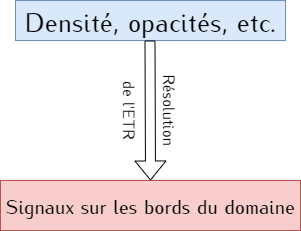
\includegraphics[width=5cm]{ProblemeDirect}       
  \end{column}

  \pause

 \begin{column}{0.5\textwidth}
    \centering
    Problème inverse \\ (\scriptsize Reconstruction de la densité par un réseau de neurones)
    %Image de signal sur les bords -> densite
      % 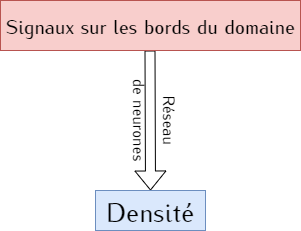
\includegraphics[width=5cm]{ProblemeInverse}       
 \end{column}
\end{columns}

\begin{figure}
  \includegraphics<1->[width=4cm]{PBInverse}         
\end{figure}

\end{frame}





\begin{frame}[fragile]
    \frametitle{Rappel des prédictions obtenues durant le stage (CNN)}

    \begin{columns}
    \begin{column}{0.5\textwidth}
        \begin{figure}
        \includegraphics<1->[width=3cm]{Meilleur2D1}       
        \includegraphics<1->[width=3cm]{Meilleur2D2}       
        \only<1-> {\caption{Les meilleures prédictions}}
        \end{figure}
     \end{column}
     \begin{column}{0.5\textwidth}
        \begin{figure}
        \includegraphics<2>[width=2.5cm]{Pire2D1}       
        \includegraphics<2>[width=2.5cm]{Pire2D2}       
        \includegraphics<2>[width=2.5cm]{Pire2D3}       
        \only<2>{\caption{Les pires prédictions}}
        \end{figure}
     \end{column}
    \end{columns}

\end{frame}

\begin{frame}
    \frametitle{Les scores obtenus par le CNN}

    \begin{table}[h!]
        \centering
        \begin{tabular}{l l}
        \toprule
        \textbf{Nom du score} & \textbf{Valeur} \\
        \midrule
        R2 & 98.81 \%\\
        Personnalisé & 93.50 \%\\
        \bottomrule\\
        \end{tabular}
    \end{table}

    \begin{columns}
        \begin{column}{0.333\textwidth}
            \begin{figure}
            \includegraphics<2->[width=2cm]{PositionX2D}       
            \only<2->{\caption{Corrélation des abscisses}}
            \end{figure}
         \end{column}
         \begin{column}{0.333\textwidth}
            \begin{figure}
            \includegraphics<3->[width=2cm]{PositionY2D}       
            \only<3->{\caption{Corrélation des ordonnées}}
            \end{figure}
         \end{column}
         \begin{column}{0.333\textwidth}
            \begin{figure}
            \includegraphics<4->[width=2cm]{Hauteur2D}       
            \only<4->{\caption{Corrélation des hauteurs}}
            \end{figure}
         \end{column}
    \end{columns}

\end{frame}


\begin{frame}
    \frametitle{Quelques mots sur la régression par le CNN}
Détection de toutes les variables :
\begin{itemize}[<+>]
    \item L'abscisse, l'ordonnée, et la hauteur sont relativement bien prédits
    \item La valeur de la densité en dehors du créneau est \textbf{fixée} :\\ $\Rightarrow$ \alert {\textbf{pas vraiment une reconstruction complète de la densité du milieu}}
\end{itemize}
\end{frame}

\setbeamercovered{invisible}

\begin{frame}
    \frametitle{Classification par CNN}
    \begin{columns}
        \begin{column}{0.65\textwidth}
            \begin{figure}
            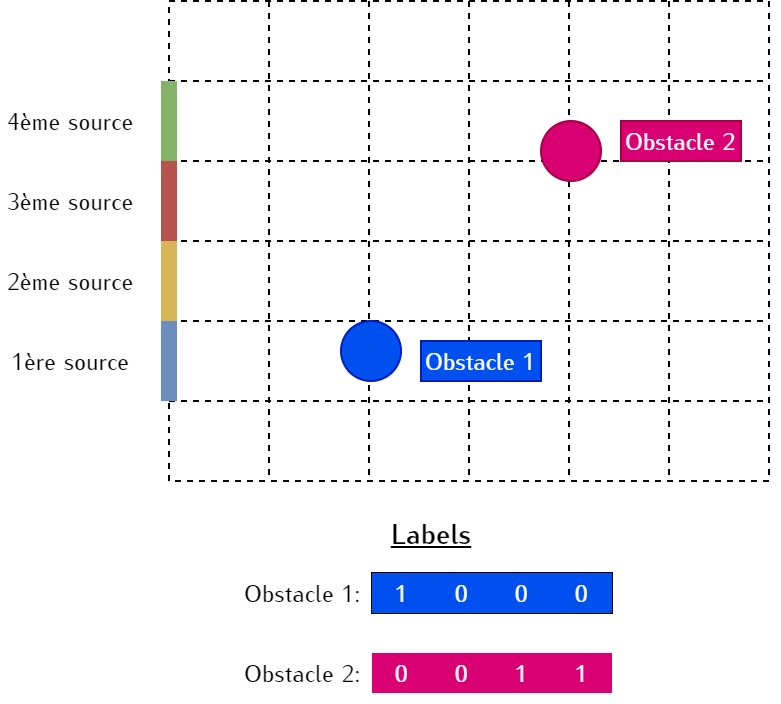
\includegraphics[width=5cm]{Classification}       
            \caption{Labels pour la classification}
            \end{figure}
         \end{column}
         \pause
         \begin{column}{0.35\textwidth}
            \begin{table}[h!]
                \caption{Les scores obtenus}
                \centering
                \begin{tabular}{l l}
                \toprule
                \textbf{Nom} & \textbf{Valeur} \\
                \midrule
                Bin. Acc. & 98.86 \%\\
                Pers. Sév. & 95.45 \%\\
                \bottomrule\\
                \end{tabular}
            \end{table}
         \end{column}
    \end{columns}
\end{frame}

\setbeamercovered{transparent}